\mbox{$\displaystyle $\,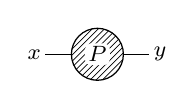
\begin{tikzpicture}[x=0.550cm, y=0.550cm, line width=0.450pt, baseline={([yshift=-0.6ex]0,0)}]
  \draw (0.000,0.000) -- (-0.600,0.000);
  \draw (0.000,0.000) -- (0.600,0.000);
  \draw (-0.600,0.000) -- (-1.200,0.000);
  \draw (0.600,0.000) -- (1.200,0.000);
  \fill[white] (0.000,0.000) circle (0.600);
  \draw[line width=0.248pt] (-0.588,0.119) -- (-0.119,0.588) (-0.599,-0.033) -- (0.033,0.599) (-0.580,-0.155) -- (0.155,0.580) (-0.541,-0.259) -- (0.259,0.541) (-0.489,-0.348) -- (0.348,0.489) (-0.424,-0.424) -- (0.424,0.424) (-0.348,-0.489) -- (0.489,0.348) (-0.259,-0.541) -- (0.541,0.259) (-0.155,-0.580) -- (0.580,0.155) (-0.033,-0.599) -- (0.599,0.033) (0.119,-0.588) -- (0.588,-0.119);
  \begin{scope}
  \clip (0.000,0.000) circle (0.600);
  \node[font=\footnotesize, inner sep=1.2pt, fill=white, rounded corners=2pt] at (0.000,0.000) {$P$};
  \end{scope}
  \draw (0.000,0.000) circle (0.600);
  \node[font=\footnotesize, inner sep=0pt, anchor=0] at (-1.290,0.000) {$x$};
  \node[font=\footnotesize, inner sep=0pt, anchor=180] at (1.290,0.000) {$y$};
\end{tikzpicture}}
\diagramgap
\mbox{$\displaystyle -\,$\,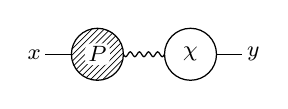
\begin{tikzpicture}[x=0.550cm, y=0.550cm, line width=0.450pt, baseline={([yshift=-0.6ex]0,0)}]
  \draw plot[smooth, tension=0.7] coordinates {(0.475,0.000) (0.449,-0.040) (0.422,-0.057) (0.396,-0.040) (0.369,0.000) (0.343,0.040) (0.317,0.057) (0.290,0.040) (0.264,0.000) (0.237,-0.040) (0.211,-0.057) (0.185,-0.040) (0.158,0.000) (0.132,0.040) (0.106,0.057) (0.079,0.040) (0.053,0.000) (0.026,-0.040) (0.000,-0.057) (-0.026,-0.040) (-0.053,0.000) (-0.079,0.040) (-0.106,0.057) (-0.132,0.040) (-0.158,0.000) (-0.185,-0.040) (-0.211,-0.057) (-0.238,-0.040) (-0.264,0.000) (-0.290,0.040) (-0.317,0.057) (-0.343,0.040) (-0.369,0.000) (-0.396,-0.040) (-0.422,-0.057) (-0.449,-0.040) (-0.475,0.000)};
  \draw (1.075,0.000) -- (0.475,0.000);
  \draw (1.075,0.000) -- (1.675,0.000);
  \draw (-1.075,0.000) -- (-1.675,0.000);
  \draw (-1.075,0.000) -- (-0.475,0.000);
  \draw (-1.675,0.000) -- (-2.275,0.000);
  \draw (1.675,0.000) -- (2.275,0.000);
  \fill[white] (1.075,0.000) circle (0.600);
  \draw (1.075,0.000) circle (0.600);
  \node[font=\footnotesize, inner sep=0.6pt] at (1.075,0.000) {$\chi$};
  \fill[white] (-1.075,0.000) circle (0.600);
  \draw[line width=0.248pt] (-1.663,0.119) -- (-1.194,0.588) (-1.674,-0.033) -- (-1.042,0.599) (-1.655,-0.155) -- (-0.920,0.580) (-1.616,-0.259) -- (-0.816,0.541) (-1.564,-0.348) -- (-0.727,0.489) (-1.499,-0.424) -- (-0.651,0.424) (-1.423,-0.489) -- (-0.586,0.348) (-1.334,-0.541) -- (-0.534,0.259) (-1.230,-0.580) -- (-0.495,0.155) (-1.108,-0.599) -- (-0.476,0.033) (-0.956,-0.588) -- (-0.487,-0.119);
  \begin{scope}
  \clip (-1.075,0.000) circle (0.600);
  \node[font=\footnotesize, inner sep=1.2pt, fill=white, rounded corners=2pt] at (-1.075,0.000) {$P$};
  \end{scope}
  \draw (-1.075,0.000) circle (0.600);
  \node[font=\footnotesize, inner sep=0pt, anchor=0] at (-2.365,0.000) {$x$};
  \node[font=\footnotesize, inner sep=0pt, anchor=180] at (2.365,0.000) {$y$};
\end{tikzpicture}}
